\documentclass[12pt]{article}
 
\usepackage[margin=1in]{geometry} 
\usepackage{amsmath,amsthm,amssymb,bm}
\usepackage{graphicx}
\usepackage[numbers]{natbib}
 
\begin{document}
  
\title{Task 4. Cloth Rendering}
\author{Garoe Dorta-Perez\\
CM50245: Computer Animation and Games II}
 
\maketitle
 
\section{Introduction}

Rendering realistic images is a challenging task, specially if there are memory or time constrains for the computation.
Cloth is a complex material composed of interwoven threads of different types.
Moreover, its appearance can vary from diffuse to highly specular.

\section{Previous work}

Several methods have been proposed to render cloth fabrics efficiently and realistically.
One of the earliest approaches was based on simple empirical shading models \cite{Weft1986}.
The main objective was to accomplish believe shading, disregarding physical accuracy.

The methods can be broadly divided into three groups, data based models, geometric models and volumetric models.

The data based approach focuses on collecting reflectance information, that will be later used to model the cloth.
Bidirectional Texture Function (BTF) \cite{Dana1999} is a function that is often used to sampled in the data based techniques.

Geometric models focus on simulation the micro-geometry of the cloth in conjunction with global illumination.
The light scattering is simulated for each fibre in the thread, where the fibres are modelled as perfect cylinders.
To be able to model the the complete scattering effects on a surface, Bidirectional Scattering-Surface Reflectance Distribution Function (BSSRDF) \cite{NicodemusFredEandRichmond1977} have been used.
With this function, complex light phenomena like subsurface scattering are modelled.

\section{Methodology}

We have chosen to implement a recent paper based on microcylinders for fast realistic cloth rendering \cite{Sadeghi2013}.
The authors proposed a model of fabric based on two microcylinders oriented in two orthogonal directions as shown in Figure \ref{fig:microcylinders}.

The reflectance of a single cylinder is defined as

\begin{equation}
L_r = \int \frac{\left(f_{r,s}(t, \omega_i, \omega_r) + f_{r,v}(t,\omega_i,\omega_r)\right)L_i(\omega_i)cos(\theta_i)\delta \omega_i}{cos^2(\theta_d)}
\label{eq:full_model}
\end{equation}

where $t$ is the thread direction, $\omega_i$ is the ray incoming direction, $\omega_r$ is the ray outgoing direction, $\theta_i, ~\theta_r, ~ \phi_i \mbox{ and } \phi_r$ are angles as shown in Figure \ref{fig:cloth_directions},  $\theta_d = \theta_i-\theta_r$ and $L_i$ is the incoming irradiance in the evaluated point.
Note that radiometric notation \cite{Marschner2003} is used to define $L_r$, which represents the outgoing radiance over a infinitesimal arc length of the cylinder and how the integral extends over the entire sphere instead of the typical hemisphere.

The surface reflection term in Equation \ref{eq:full_model} is defined as

\begin{equation}
f_{r,s}(t, \omega_i, \omega_r) = F_r(\eta, \omega_i) cos(\phi_d/2)g(\gamma_s, \theta_h)
\end{equation}

where $\theta_h = (\theta_i+\theta_r)/2$, $\phi_d = \phi_i-\phi_r$, $F_r$ is a Fresnel reflection term that is computed using \citeauthor{Schlick1994}'s approximation \cite{Schlick1994} $F_r(\eta, \omega) = \eta + (1 - \eta)(1 - h \cdot \omega)^5$ where $h = (\omega_r + \omega_i)/ \left|\omega_r + \omega_i \right|$ is the normalized halfway vector and $\eta$ is the reflectance for $h \cdot \omega = 1$, $g(\gamma, \theta) = \gamma e ^{p-1}$ is a Gaussian lobe \cite{Wang2008} where $p$ is the lobe axis, $\lambda$ is the sharpness, the direction $v$ is the spherical parameter in the resulting function and $\gamma$ is the amplitude.

The volume scattering term in Equation \ref{eq:full_model} is defined as

\begin{equation}
f_{r,v}(t,\omega_i,\omega_r) = F_t(\eta, \omega_i) F_t(\eta', \omega_r') \frac{(1-k_d)g(\gamma_v, \theta_h)+k_d}{cos(\theta_i) + cos(\theta_r)} A
\end{equation}

where $k_d$ is a scattering constant, $A$ is a albedo constant, $F_t = 1 - F_r$ is a Fresnel transmission term, $\omega_r'$ is a projection of $\omega_r$ into a plane that contains the normal $n$ and $\eta'$ is computed using the Bravais index \cite{Marschner2003} as $\eta'(m) = \sqrt{\eta^2 - sin^2(m)}  / cos(m)$ where $m$ is the angle between $\omega_r$ and its projection $\omega_r'$.

\begin{figure}[ht!]
\begin{minipage}[b]{.45\textwidth}
\centering
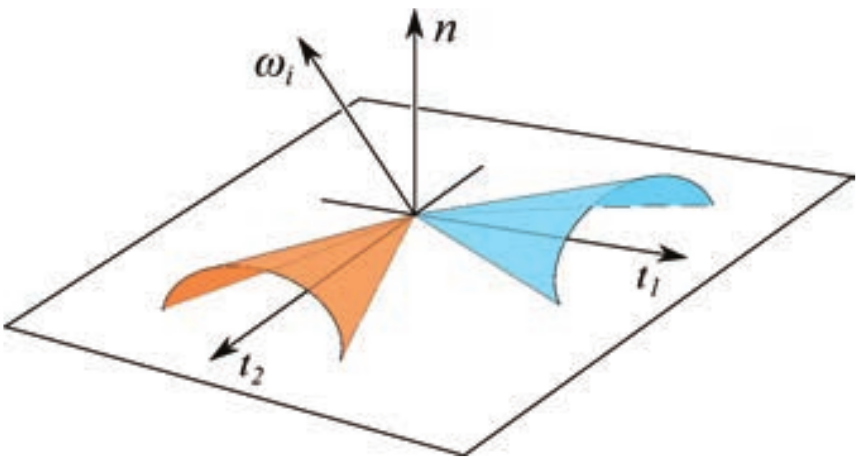
\includegraphics[width=1\textwidth]{images/microcylinders}
	\caption{\citeauthor{Sadeghi2013} shading model \cite{Sadeghi2013}, where $\omega_i$ is the incident light direction, $n$ is the surface normal and $t_1,t_2$ are the orthogonal thread directions.}
	\label{fig:microcylinders}
\end{minipage}
\hfill
\begin{minipage}[b]{.45\textwidth}
\centering
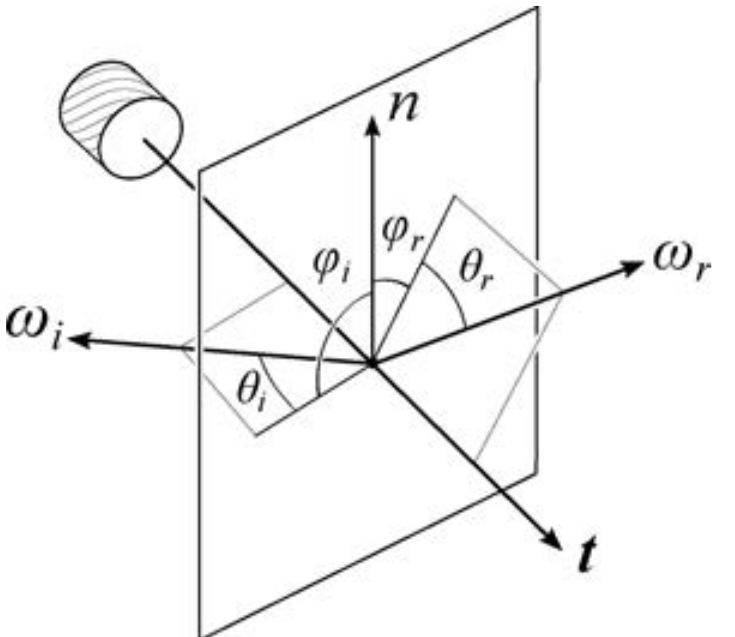
\includegraphics[width=1\textwidth]{images/cloth_directions}
	\caption{\citeauthor{Sadeghi2013} shading model \cite{Sadeghi2013}, showing $\theta$ and $\phi$ angles given a pair of directions $\omega_i$ and $\omega_r$.}
	\label{fig:cloth_directions}
\end{minipage}
\end{figure}

\section{Results}

\section{Conclusion and Future Work}

\bibliographystyle{plainnat}
\bibliography{t4_report}

\end{document}

